\chapter{Week 7}

\section{Support Vector Machines}

\subsection{Alternate view of logistic regression}

\[ \hth(x) = \frac{1}{1 + e^{-\theta^T x}} \]

Ideally, if $y=1$, we would like $\hth(x) \approx 1$, so we want $\theta^T x \gg 0$.
Likewise, if $y=0$, we want $\theta^T x \ll 0$.

Each example contributes the following cost:

\[ - \qty( y \log(\hth(x)) + (1-y)\log(1-\hth(x)) ) \]

The first term only applies when $y=1$ and the second term only applies when $y=0$.

For a SVM, we modify this cost term to be
flat at 0 (no cost) when the decision is correct,
and to grow linearly the more the decision is incorrect.
(The slope doesn't matter much.)

\begin{center}
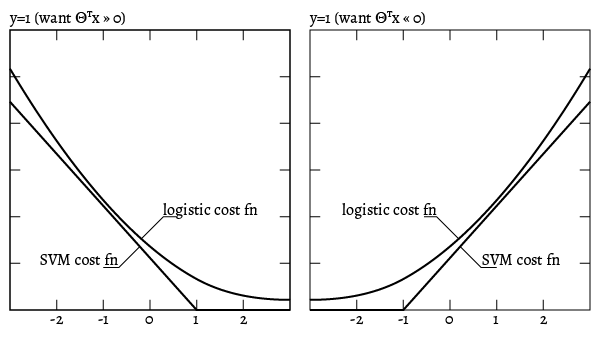
\includegraphics[width=4in]{images/svm-cost-function.png}
\end{center}

Notation: these cost functions are called $\cost_1(z)$ for the $y=1$ case,
and $\cost_0(z)$ for the $y=0$ case.
So a Support Vector Machine has a cost function:

\[ 
    \min_\theta C 
    \sum_{i=1}^m \qty[
        y\s{i} \cost_1(\theta^T x\s{i}) + 
        (1-y\s{i}) \cost_0(\theta^T x\s{i}) 
    ]
    + \frac{1}{2} \sum_{j=0}^n \theta_j^2
\]

By convention, we exclude the factor of $\frac{1}{m}$ from the cost function,
and we use $C$ as the regularization parameter.
That is, we minimize $CA + B$ rather than $A + \lambda B$.
So a small $C$ weighs regularization heavily,
while a large $C$ weighs fitting the training set heavily.
(Think of $C \approx \frac{1}{\lambda}$).

Unlike logistic regression, an SVM does not output a probability.

\[
    \hth(x) = \begin{cases}
        1 \text{ if } \theta^T x \geq 0 \\
        0 \text{ if } \theta^T x < 0
    \end{cases}
\]

\subsection{Large Margin Intuition}

$\cost_1(z)$ is 0 only when $z \geq 1$,
even though we have classified correctly whenever $z \geq 0$.
Likewise, $\cost_0(z)$ is 0 only when $z \leq -1$,
even though we have classified correctly whenever $z < 0$.
Consequently, we want not just to barely get the examples right,
but to have a significant margin of correctness.

Imagine $C$ is extremely large, so we weigh fitting the data very highly.
So whenever $y\s{i} = 1$ we want $\theta^T x \geq 1$,
and whenever $y\s{i} = 0$ we want $\theta^T x \leq -1$.
Since $C$ is so large, we will probably reject any hypothesis which
incorrectly classifies any examples,
so we are left minimizing only the regularization term.

For a linearly separable case, this will draw a decision boundary which
has the largest possible margin between the boundary and the closest points.

For very large $C$, the SVM is very sensitive to outliers,
and might drastically change the boundary to accommodate a single point.
Regularization prevents this.

\subsection{Mathematics behind large margin classification}

Consider $u = \mqty(u_1 \\ u_2)$ and $v = \mqty(v_1 \\ v_2)$.
Then the inner product $u^T v$ is $u_1 v_1 + u_2 v_2$.
And $\norm{u} = \sqrt{u_1^2 + u_2^2}$.
We also have $u^T v = \mathrm{proj}_u(v) \cdot \norm{u} = \mathrm{proj}_v(u) \cdot \norm{v}$.

For the SVM decision boundary, we are effectively minimizing

\[
    \min_\theta \frac{1}{2} \sum_{j=1}^n \theta_j^2  
    \quad \text{ such that } \quad
    \theta^T x\s{i} \geq 1 \text{ if } y\s{i}=1
    \quad \text{ and } \quad
    \theta^T x\s{i} \leq -1 \text{ if } y\s{i}=0
\]

Assume $\theta_0 = 0$.
In the case where $n=2$, we are minimizing $\theta_1^2 + \theta_2^2$,
or equivalently, $\qty(\sqrt{\theta_1^2 + \theta_2^2})^2$, which is $\norm{\theta}^2$.

Now consider $\theta^T x\s{i}$.  This can be thought of as the projection of $x\s{i}$
onto the parameter vector $\theta$ times $\norm{\theta}$.
So we are really finding:

\[
    \min_\theta \frac{1}{2} \norm{\theta}^2
    \quad \text{ such that } \quad
    \mathrm{proj}_\theta x\s{i} \cdot \norm{\theta} \geq 1 \text{ if } y\s{i}=1
    \quad \text{ and } \quad
    \mathrm{proj}_\theta x\s{i} \cdot \norm{\theta} \leq -1 \text{ if } y\s{i}=0
\]

Simplifying notation: let $p\s{i} = \mathrm{proj}_\theta x\s{i}$

This all makes sense if $\theta$ is a vector orthogonal to the decision boundary.
The projections of $x\s{i}$ onto $\theta$ are the distances to the decision boundary,
and we require these all to be above 1.

If the boundary is bad (small margins), then $p\s{i}$ is small,
so by our condition above, $\norm{\theta}$ must be large
(in order for the product to be greater than 1).
Since we're trying to minimize $\norm{\theta}^2$, our algorithm will not choose such a boundary.

Removing the assumption that $\theta_0=0$ just allows us to have 
decision boundaries that do not pass through the origin.
It is just somewhat less obvious to show that this leads to a large margin classifier.

\section{Kernels}

Kernels adapt SVMs to support non-linear models.
One way is to include polynomial features.
This would look like:

\[
    \text{Predict } y=1 \text{ if } \quad
    \theta_0 + \theta_1 x_1 + \theta_2 x_2 + \theta_3 x_1 x_2 + \theta_4 x_1^2 + \dots \geq 0
\]

Instead we can write this more generally as 

\[
    \theta_0 + \theta_1 f_1 + \theta_2 f_2 + \theta_3 f_3 + \theta_4 f_4 + \dots \geq 0
\]

\[
    \theta^T f \geq 0
\]

Where $f$ is the new set of features.  But $f$ doesn't have to come from polynomial features.

Example: compute new features based on proximity to landmark points $l\s{1}, l\s{2}, l\s{3}$.
So $f_j = \text{similarity}\qty(x,l\s{j})$.
We can use a similarity metric like:

\[
    \text{similarity}\qty(x,l\s{j}) = \exp(-\frac{\norm{x-l\s{j}}^2}{2\sigma^2})
\]

The similarity function is called a kernel, and this particular function is called a Gaussian kernel.
It has the feature that $f \approx 1$ when $x \approx l$, and $f \approx 0$ when $x$ is far from $l$.
When $\theta_j$ has a positive value, the classifier will predict 1 for points sufficiently close to
the landmark point $l\s{j}$.

But how do we choose the landmark points $l$?  And what other similarity functions work?

One choice of how to choose $l$ is to use $l\s{i} = x\s{i}$ for $i$ from 1 to $m$.
So you would have as many features as training examples (plus 1 for $\theta_0$),
and the data matrix would become a similarity matrix.
So $X_{ij} = \text{similarity}\qty(x\s{i}, x\s{j})$.

This is a lot of features, but it's way fewer than you would get by adding many polynomial features.

An additional detail: the regularization term $\frac{1}{2} \sum_{i=1}^m \theta_j^2 = \theta^T \theta$
is typically replaced by $\theta^T M \theta$ where $M$ is some matrix that depends on the kernel.
This is done mostly for computational efficiency.

Kernels could be used for other learning methods, but it turns out to be more efficient for SVMs
than for something like logistic regression.

\section{SVM hyperparameters}

Choosing $C$ trades off between bias and variance

Choosing $\sigma^2$ causes features $f_i$ to vary more smoothly,
resulting in higher bias and lower variance.

\section{Using an SVM}

Use a SVM software package to solve for parameters $\theta$

Need to specify $C$ and the kernal.
No kernel is called a ``linear kernel''.  This is okay if $n$ is large, or $m$ is small.
If you choose a Gaussian kernel, you must also specify $\sigma^2$.

You should perform feature scaling before using the Gaussian kernel;
otherwise, larger-valued features will dominate in $\norm{x-l}$.

Any kernel must satisfy a condition called ``Mercer's Theorem''.
A second example is the polynomial kernel:
$k(x,l) = (x^T l + \text{constant})^\text{degree}$,
but this generally performs worse than the Gaussian kernel.
However, sometimes it makes sense for non-negative data.
More rare:

\begin{itemize}
    \item String kernel
    \item Chi-square kernel
    \item Histogram intersection kernel
\end{itemize}

\subsection{Multi-class Classification}

One option is the one-vs-all method
(train $K$ SVMs for $K$ classes, 
get $\theta\s{1}\dots\theta\s{K}$, 
and pick the class with the largest $\theta^T x$).

The other option is just to use the built-in multi-class utility
in the software package you're using.

\subsection{Logistic Regression vs. SVM}

\begin{itemize}
    \item If $n \gg m$
        use logistic regression or a SVM with a linear kernel
    \item If $n$ is small and $m$ is intermediate (10-10,000),
        use a SVM with a Gaussian kernel
    \item If $n$ is small and $m$ is large (50,000+), add more features
        and use logistic regression or an SVM with a linear kernel
\end{itemize}

Neural networks will probably work well for many of these scenarios, 
but may be slower to train.

SVMs have the benefit of convexity, so they will always find a global minimum.